\documentclass[11pt, letterpaper]{article}  % change to >11 pt if you like, and change article with report
\usepackage[letterpaper, top=3.71cm, bottom=3.20cm, left=2.86cm, right=2.86cm]{geometry}
\usepackage[utf8]{inputenc}
\usepackage{natbib}
\usepackage{graphicx}
\usepackage{color}
\usepackage{subfig}
\usepackage{float}
\usepackage{hyperref}
\usepackage{url}
%\usepackage{pythontex}
\definecolor{bg}{gray}{0.95}
\usepackage{minted}
\usepackage{wrapfig}

\title{\vspace{-2cm}\textbf{Data Mining project report}}
\author{\textbf{\small{\textit{Dalla Noce Niko, Ristori Alessandro, Giuseppe Lombardi}}} \\ % put your full name here
        \small{Master Degree in Computer science.}\\ \small{{n.dallanoce@studenti.unipi.it, a.ristori5@studenti.unipi.it, g.lombardi11@studenti.unipi.it}.} \\  % put your Master Degree here
        \small{Data Mining, Academic Year: 2021/2022} \\
        \small{Date: 10/11/2021} \\
       \textbf{\small{\url{https://github.com/nikodallanoce/DataMiningProject}}}
}

\renewcommand\refname{} %remove this line to automatically show the bibliography header

\begin{document}

\nocite{*}  % comment this line to list only the articles you really cite
\date{}
\maketitle
\begin{center}
    
\includegraphics[width=0.2\textwidth]{images/unipi.png}\\
    \vspace{0.5cm}
\end{center}
%\begin{abstract}
%The report starts with a long, but needed introduction to the main concepts that we've seen during the course of our work and it shows what was our purpose and how we reached it. Then it shows the results obtained by the models we tried giving at the same time the reasons of their performances. The report concludes with our final considerations on what and how we could have done more.
%\end{abstract}
\newpage
\tableofcontents
\newpage
%\listoffigures
%\section{Introduction}

\section{Data understanding and preparation}
We focused our work on the matches dataset that contains tennis matches played in many tournaments across the world over the last five years, it includes both male and female players and has 186.129 records and 49 features. We decided not to do any cleaning or integration on the male and female datasets since they were only used to get the sex for each player.

\subsection{Data understanding}
The data understanding task focuses on analyzing the dataset and its integration by removing duplicated values, fixing missing values and solving the possible outliers.
\subsubsection{Data semantics}
In this phase we focused on understanding the meaning of each feature inside the dataset.
\begin{itemize}
    \item \textbf{tourney\_id}: it's a \textit{string} that uniquely identifies each tournament. It is mainly composed by two parts separated by a dash "-", where the first one indicates the year when the tournament was played and the second one refers to the tournament identifier, i.e. '2018-W-WITF-EGY-03A-2018'. The dataset contains some null value for this feature (only for the last tournament), while it has 4853 unique values.
    \item \textbf{tourney\_name}: it's a \textit{string} that represent the name of the tournament and it's not unique because the name of the tournament is usually the same over the years. It has some missing values only in the last part of the dataset.
    \item \textbf{surface}: it indicates the surface where the matches took place. It's a categorical attribute which its possible values are: hard, clay, grass and carpet. Only few matches are missing this feature.
    \item \textbf{draw\_size}: it's a \textit{float} that indicates the number of players in a tournament.
    \item \textbf{tourney\_level}: it's a \textit{string} indicates whether the tournament is for male or female players and also its level (mastr, ATP500, ATP1000 etc.). Has some missing values in the last part of the dataset just like for the tourney\_id.
    \item \textbf{tourney\_date}: it's the date when the match took place. In the dataset it's a \textit{float} in the form YYYYMMDD. To use it as real date, a parsing to a date type is needed. Missing values are present only in the last part of the dataset.
    \item \textbf{match\_number}: it's a \textit{float} number that represents the match number in a tournament. Due to its meaning, it should be parsed to an integer.
    \item \textbf{winner\_id}: it's a \textit{float} representing the id of the match winner. It's unique for players with the same gender, while the same id can appear for a male player and for a female player as well, since they play in different tours (ATP and WTA).
    \item \textbf{winner\_entry}: it's a \textit{string} that indicates how a player joined the tournament. There are a lot of missing values for this feature.
    \item \textbf{winner\_hand}: it's a \textit{string} representing the winner player's favourite hand. Its possible values are 'U' for unknown, 'R' for right and 'L' for left. Actually there are also null values, but they can be treated as unknown.
    \item \textbf{winner\_ht and loser\_ht}: \textit{float} representing the winner player's height. There are a lot of missing values for this field that can not be inferred by other records where this it's filled.
    \item \textbf{winner\_ioc and loser\_ioc}: a 3-character \textit{string} representing the player's nationality. Some of them have been written using different standards. For instance, a German player is present both as 'GER' and as 'DEU'. Also, some players appear with more than one nationality because they switched it during the last years.
    \item \textbf{winner\_age and loser\_age}: a \textit{float} that indicates the age of the winner. The decimal part represents the percentage of the days days left to the birthday. Some of these values are missing in the dataset, but few of them can be precisely inferred.
    \item \textbf{best\_of}: a \textit{float} indicating the number of set for a match. We parse it to an integer.
    \item \textbf{round}: the match round (e.g. F stands for final and SF for semifinal).
    \item \textbf{minutes}: indicates how much a match lasted. It's a \textit{float} that we converted to an integer.
    \item \textbf{w\_ace and l\_ace}: number of aces (valid serve won, first or second, not touched by the opposing player). It's a \textit{float}, but it should be an integer.
    \item \textbf{w\_df and l\_df}: number of double faults committed by the player (more specifically the number of invalid second serves). It's a \textit{float} converted to int.
    \item \textbf{w\_svpt and l\_svpt}: this may be confusing, it isn't the number of points obtained after a player's serve but the number of serves done by the player (the former is referred on specialised sites as serve points won).
    \item \textbf{w\_1stIn and l\_2stIn}: number of valid first serve by the player.
    \item \textbf{w\_1stWon and l\_1stWon}: number of points won after a valid first serve by the player.
    \item \textbf{w\_2ndWon and l\_2ndWon}: number of points won after a valid second serve by the player, be aware that a point lost after a second serve could be a double fault (this means that the second serve wasn't valid).
    \item \textbf{w\_SvGms and l\_SvGms}: number of games (not points) where the player was serving.
    \item \textbf{w\_bpSaved and l\_bpSaved}: number of breakpoints (the player is a point from losing a game where he's serving) saved (the player serving won the point).
    \item \textbf{w\_bpFaced and l\_bpFaced}: number of breakpoints that the player faced (see previous feature).
    \item \textbf{w\_rank and l\_rank}: the player's rank, in tennis points are awarded based on the performance at each tournament.
    \item \textbf{w\_rank\_points and l\_rank\_points}: the player's ranking points.
    \item \textbf{tourney\_revenue}: the tourney revenue coming from ticket sales etc. It isn't the prize of the tournament (which would have been more interesting for a player analysis).
    \item \textbf{tourney\_spectators}: number of spectators of the entire tournament.
\end{itemize}

\subsubsection{Type casting}
In this dataset, most of the features have an incorrect data type. We parse the tourney\_date from float to pandas date type. Furthermore, every float attribute has been parsed to integer except for the winner/loser age and the tourney\_revenue.

\subsubsection{Dropping useless matches}
There are many matches without any statistics, highlighted in \autoref{fig:features_heatmap}. Such matches are from minor tournaments and the players who played in them don't have many matches in the dataset, we decided to drop them.
\begin{figure}[H]
    \centering
    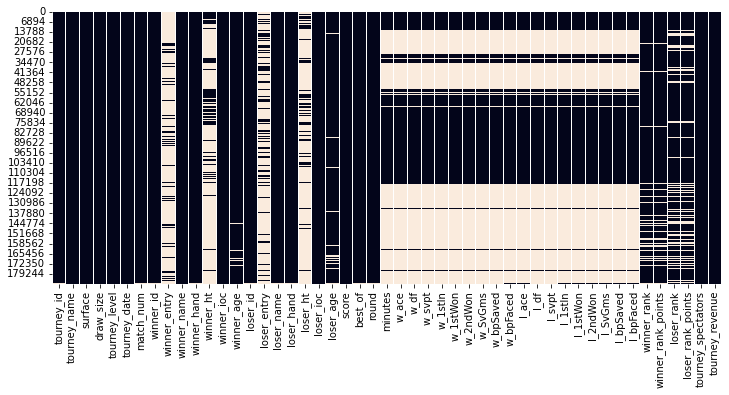
\includegraphics[width= 0.6\linewidth]{images/data_understanding/feature_heatmap.png}
    \caption{The missing values heatmap.}
    \label{fig:features_heatmap}
\end{figure}
Furthermore, starting from line n. 186073 to the end, we found a block of records that is a copy of some matches of the Taipei tournament, but with some field left empty. Having noticed this, we dropped this useless part of the dataset.

\subsubsection{Dropping useless features:}
For our purpose, an analysis of the players, some features are not interesting or straight useless, so we decided to drop them. We don't need the \textbf{tourney name}, since we don't differentiate between the tournaments (masters atp, ATP1000 etc.), moreover we already have the \textbf{tourney id} and \textbf{date}.

The \textbf{draw size} is useless for the players and the \textbf{tourney level} can't be used to differentiate between men and women, since the latter can play the same kind of tournaments of the former. For what concerns \textbf{match num}, it's a progressive number for the matches of a tournament, sometimes is totally arbitrary, we don't need it.

\textbf{Winner entry} (and \textbf{loser entry}) is a string that shows if the player qualified by a wildcard, as a lucky loser etc., it's not a very useful attribute since no site lists them, moreover is the feature with the most missing values.

The last features we dropped are \textbf{tourney revenue} and \textbf{tourney spectators}, the former is the amount of revenue generated by the tournament and not the winner prize which would have been really interesting. The latter is the amount of spectators of the entire tournament, not match to match, so we can't retrieve information about how famous the players involved in a certain match are or if they can play better under more pressure.

\subsubsection{Dropping duplicates}
We found that the matches dataset has 302 duplicated records. Due to the domain of this dataset, these duplicates are useless, so we dropped them.

\subsubsection{Data integration}
The data integration task consists in solving the various issues found in the dataset by filling the missing values, where it's possible, and fixing the various problems that may arise (e.g.: players with two hands preferred or with more than one ioc).
\paragraph{Player id and name}
In our analysis, we found that there are three players ('Guy Stokman', 'Giuseppe Tresca', 'Kuan Yi Lee') that appear in the dataset with more than one id associated. Moreover, there's only one player with an actual homonym (Kuan Yi Lee), one is a male (id: 134120) and the other one is female (id: 221745), but we discovered that the actual name of the male player is Kuan-Yi, so we changed his name to differentiate between the two players. For what concerns the other two players, we assigned them their last id.

Deepening the analysis, we found that ids are shared only between a male and female player and this is allowed since different tours exist (ATP and WTA) for each sex, so we don't need to apply any change, moreover we won't work with ids so this won't affect our analysis.

\paragraph{Surface}
We found that the "surface" feature has some null values. Moreover, the number of tournaments without a surface are 42 while the number of matches without a surface are 117. In order to solve this problem, for those tournaments that lack the surface  we can retrieve it if at least one match of the same tournament has it. Unluckily there are no tournaments for which we could retrieve the surface (all of them are from the Davis or Federation cup, where the surface changes from event to event), so we chose to sample such values from the distribution of the surfaces.

\paragraph{Winner/loser hand}
We have to manage the missing values for both "winner\_hand" and "loser\_hand". To do this, we checked if the value is missing only for a particular player or if he/she never has the hand defined and, in this case, we assign it to him/her. After this step, however, the missing values are still present, but since the domain of this feature is {'U', 'L', 'R'}, we can safely treat null values as 'U'. The players with unknown hand are 1840. Among them, we retrieved the actual preferred hand for one player, Amina Anshba, who is left-handed.

\paragraph{Winner/loser height}
This feature contains missing values too, so we addressed this problem as before, looking for those players that have a known height somewhere in the dataset. A deeper analysis show us that 'David Goffin' has two heights registered: 180 cm and 163 cm. Since his real height is the first one, we fixed it in in all occurrences in which he appears.

\paragraph{Winner/loser ioc}
Since there are no missing values for this feature, we only needed to check if there are players with more than one ioc. Since we dropped records and players that have played too few matches, we haven't found players with more than one ioc. In the original dataset, instead, it happens. Anyway, we found that the player called 'Xinmu Zhou', has 'UNK' nationality, but he is Chinese actually, so we assign him 'CHN'. Lastly, we discovered that, sometimes, the acronyms of the nations are wrong, since some of them don't follow the international standard (e.g.: GRE for Greece instead of GRC, or TPE for Taiwan instead of TWN) or have both at the same time (e.g.: DEU and GER for Germany), so we fixed them, at least the ones we found.

\paragraph{Winner/loser age}
There are 58 players with unknown age. Among them there are only two players whose age can be inferred from the other information inside the dataset, we fixed the missing ages during the data preparation task. 

\paragraph{Winner/loser rank} This information is missing for those players that played only few matches. We fixed the missing values with the last tournament rank for each player (or the next if not present) that already had a rank. For those without rank we assumed they didn't have any points so we assigned them the maximum rank found in the dataset.

\paragraph{Winner/loser rank points} Same work as for the rank feature, instead this time we assign the minimum value for those players without any rank points (they are the same we found during the rank integration).

\subsubsection{Outlier detection}
Given that all the feature distribution are Gaussian or half normal, to analyze outliers we must first compute the first quartile, the third quartile, the median and the interquartile for each feature. Then we compute the lower bound $L=Q1 - 1.5 * IQR$ and the upper bound $U=Q1 + 1.5 * IQR$ for each feature. In case some numerical data was less or greater than the lower or upper bound respectively, we can identify an outlier. For half-normal distribution we don't consider the lower bound. In case of an outlier that can be fixed with a real value, we did it. In this way we found, for example, two players that have too low height and, in fact, these data were wrong. We fixed it with the players' real height. Whereas high values correspond to those players that are actually tall. We have applied this analysis for every numerical feature.
\begin{figure}[H]
    \centering
    \subfloat[Before detection]{{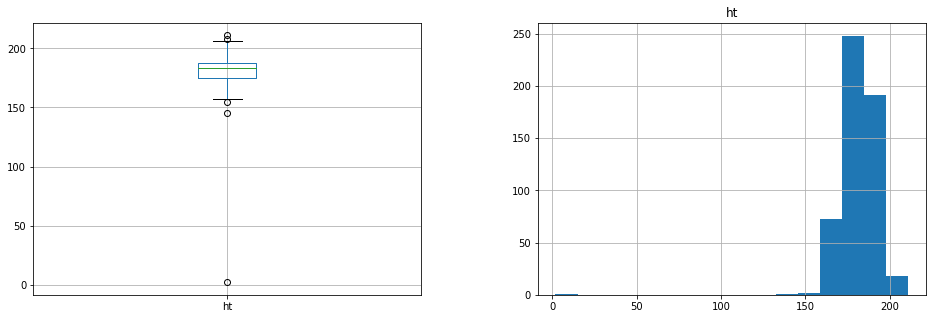
\includegraphics[width= 0.5\linewidth]{images/data_understanding/ht_before_detection.png}}}%
    \subfloat[After detection]{{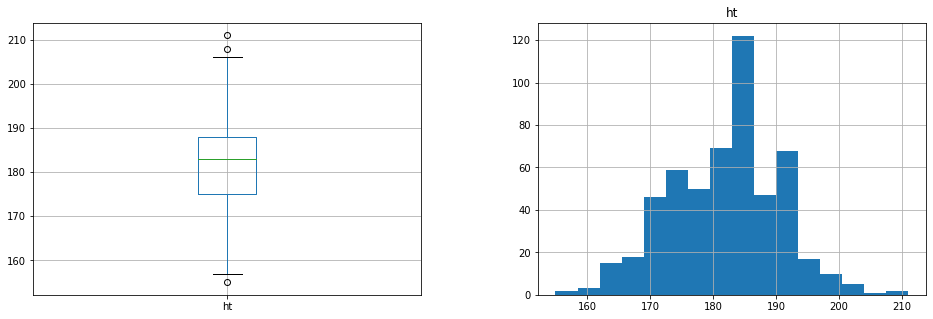
\includegraphics[width= 0.5\linewidth]{images/data_understanding/ht_after_detection.png}}}%
    \caption{An example of a feature's distribution after dealing with outliers.}
    \label{fig:before_and_after_detection}
\end{figure}

\subsubsection{Correlations}
We plotted the correlation matrix in order to visualize whether there are correlations between the features. In \autoref{fig:corr_matrix_tennis_matches}, the more the color is red the more the features are correlated.
\begin{figure}[H]
    \centering
    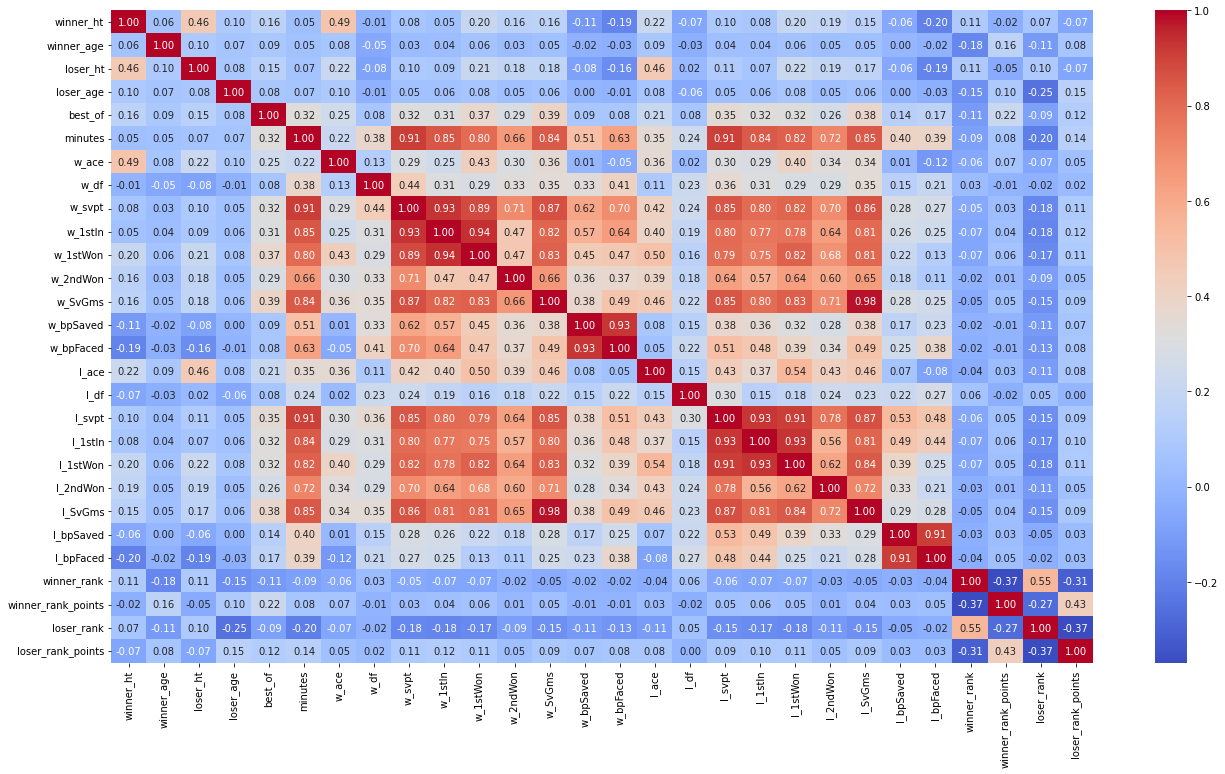
\includegraphics[width= 0.8\linewidth]{images/data_understanding/correlation.png}
    \caption{Correlation matrix of the tennis matches dataset.}
    \label{fig:corr_matrix_tennis_matches}
\end{figure}
After looking at the correlation matrix we dropped the minutes feature since we deemed it as useless after doing a huge help during the outlier detection by showing "inusual matches". 
\subsection{Data preparation}
In this section we focus on describing how we built our new dataset, cleaned and composed by some new features derived by the original ones.

\subsubsection{Building the player's profile}
The purpose of data preparation is building a profile that will feed the clustering analysis, as a starting point we decided to build such profile from the features we had from the matches dataset.

\paragraph{Sex}
First of all, when we started building our new dataset, we assigned the sex to each player inside tennis\_matches using the female\_players and male\_players datasets. Some players of the tennis\_matches dataset were not found in the "sex" dataset due to spelling errors in their name, but we solved this problem by looking online.
\begin{figure}[H]
    \centering
    \subfloat[Sex distribution]{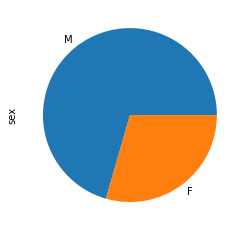
\includegraphics[width=0.20\linewidth]{images/data_preparation/sex_distribution.png}}
    \subfloat[Age distribution]{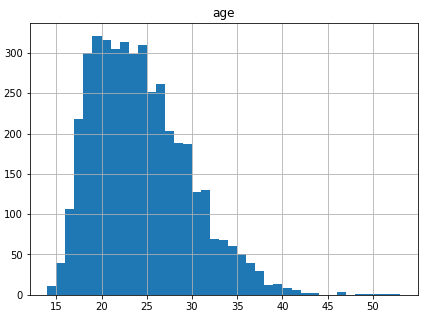
\includegraphics[width=0.25\linewidth]{images/data_preparation/age_distribution.png}}
    \caption{Sex and age distribution}
    \label{fig:sex_age_feature}
\end{figure}
\paragraph{Age}
Since we are doing a "current" analysis, we assign to each one of the players the last age they appear in the original dataset. Some of them have an unknown one, we had to sample it.

\paragraph{Ioc} This was the easiest one since we didn't have to deal with missing values.
\begin{figure}[H]
    \centering
    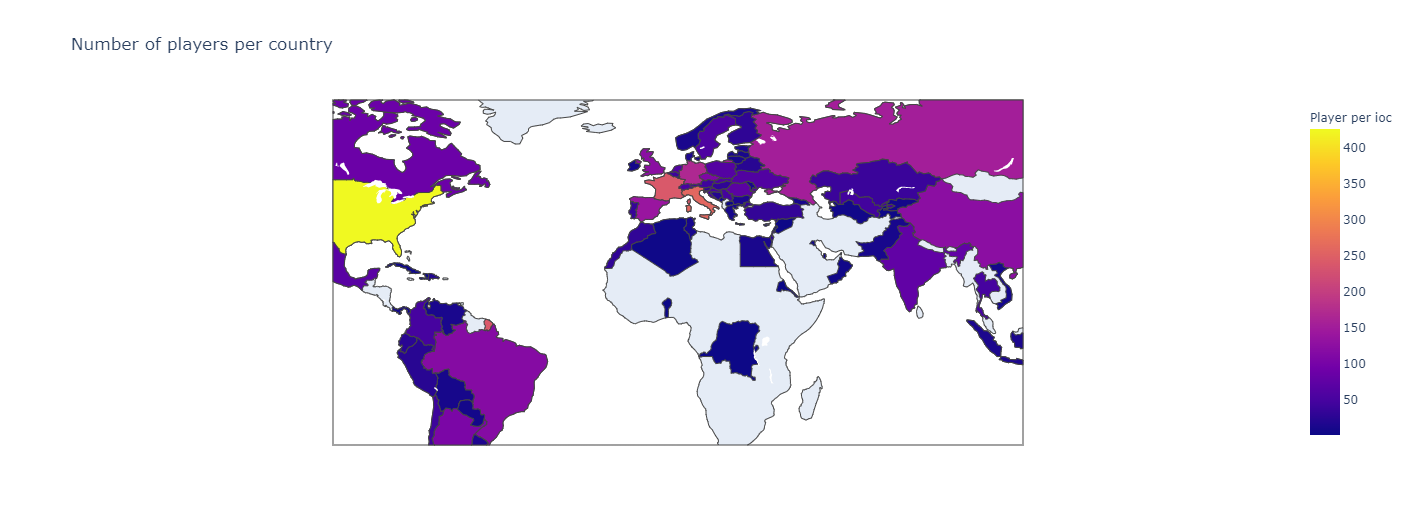
\includegraphics[width=0.74\linewidth]{images/data_preparation/ioc_distribution.png}
    \caption{IOC distribution}
    \label{fig:ioc_feature}
\end{figure}

\paragraph{Height} We solved the issue of having many players without an height by sampling their height from the distributions based on countries and sex where this was possible, otherwise we assigned them the mean height of their respective sex.

\paragraph{Hand} Just like for the ioc we just needed to assign the hand to the players since the missing values were already dealt with.

\paragraph{Wins and losses} We calculated the total matches won or lost by the player and also how many matches they won on a specific surface.

\paragraph{Tournaments won} We calculated the tournaments won by the player by looking at how many times he appeared in a final as the winner.

\paragraph{Surfaces} We inserted the amount of wins by a player for each surface he/she played on, moreover we dropped all the statistics (percentage of win and number of wins) about the matches played on carpet since such surface is no more allowed by the international federation.

\paragraph{Statistics, rank and rank points} For each player we calculated all the statistics coming from the cleaned matches dataset, futhermore we assigned at each player their rank and rank points, eliminating from the dataframe those that played less than ten matches.

\subsubsection{Building new features}
\iffalse
\begin{figure}[H]
    \centering
    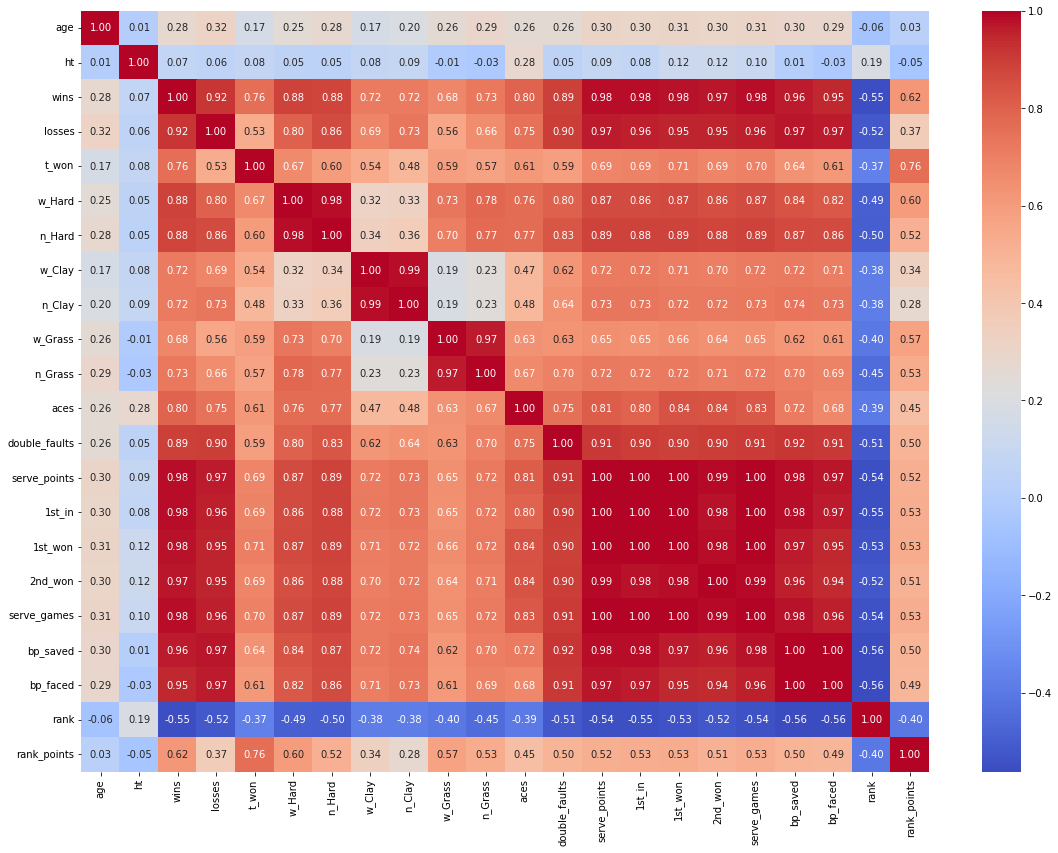
\includegraphics[width= 0.59\linewidth]{images/data_preparation/correlations_before_new_features.png}
    \caption{Correlation matrix of the new dataset with the features coming from the matches dataset.}
    \label{fig:corr_matrix_old_features}
\end{figure}

As we can see from \autoref{fig:corr_matrix_old_features},\fi
Having inserted the features coming from the cleaned matches dataset, it was time to look at the correlations between those features, we saw that many of those were many highly-correlated, so we decided to build new ones from them, such as [\textit{num\_matches, p\_wins, p\_w\_Hard, p\_w\_Clay, p\_w\_Grass, mean\_ace and p\_aces, mean\_double\_faults and p\_double\_faults, mean\_1st\_in and p\_1st\_in, mean\_1st\_won and p\_1st\_won, mean\_2nd\_won and p\_2nd\_won,\\mean\_bp\_saved and p\_bp\_saved, mean\_bp\_faced, mean\_sv\_games, mean\_sv\_points}]

\paragraph{Categorical features} We built categorical attributes that split players by age, height and rank ranges.
\vspace{3mm}

We then dropped the features that were too high correlated with another one or we deemed useless for the players analysis (n\_matches, mean\_aces, mean\_sv\_games, mean\_double\_faults).
After adding the new derived features, we checked that they were not correlated each other by calculating again the correlation matrix, as showed in \autoref{fig:corr_matrix_new_ds}.

\begin{figure}[H]
    \centering
    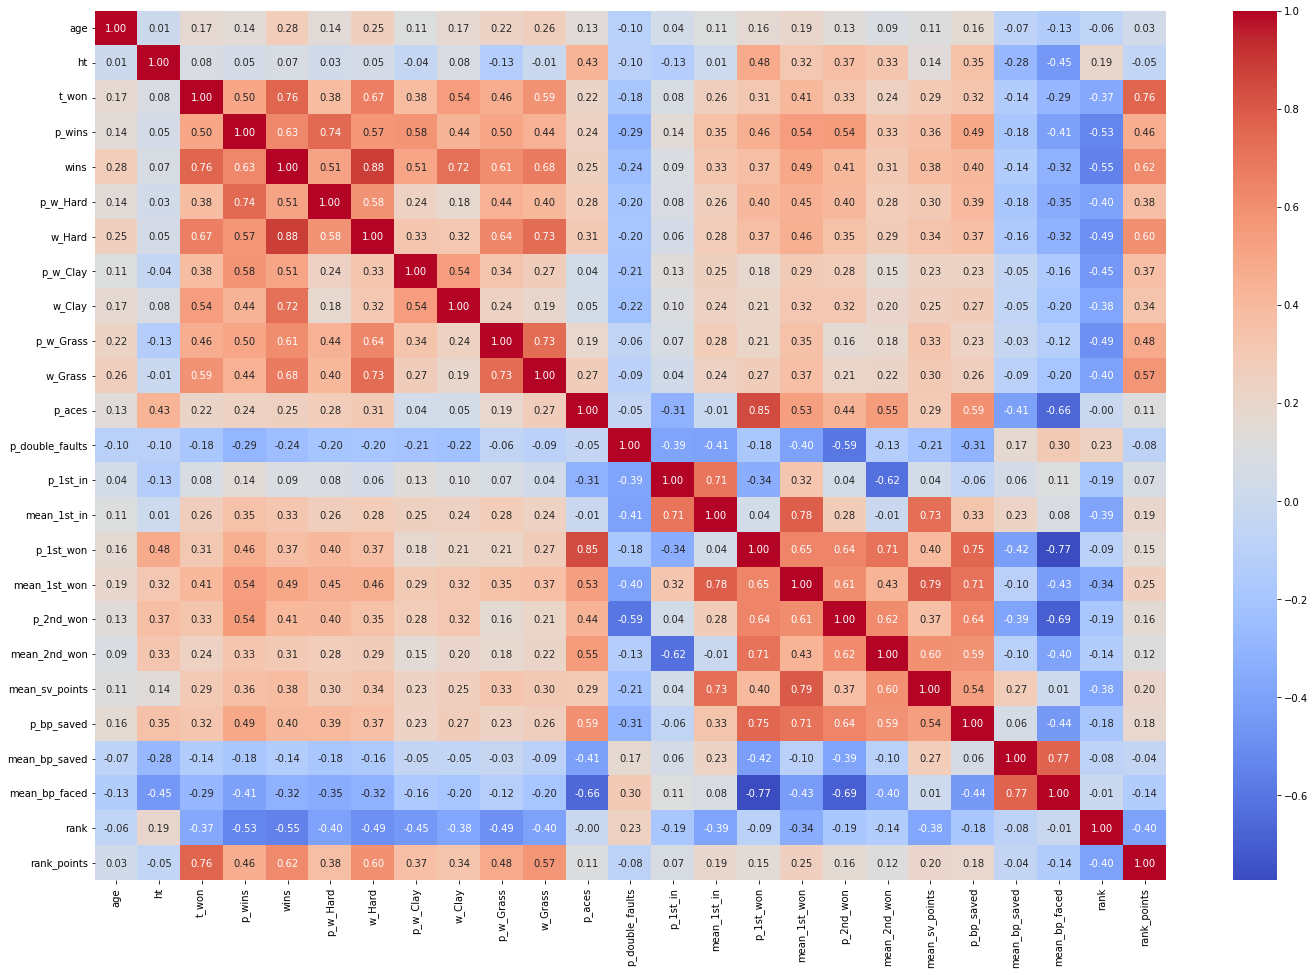
\includegraphics[width=0.8\linewidth]{images/data_preparation/players_corr_features.png}
    \caption{Correlation matrix of the new dataset with the features we added.}
    \label{fig:corr_matrix_new_ds}
\end{figure}
\section{Clustering analysis}
\subsection{Preprocessing}
In order to let the cluster algorithms work, we had to preprocess the data. Initially we tried to use the MinMax scaler, but we saw that K-Means was not working well. Due to that, we decided to normalize such features with their z-score by using the scikit-learn StandardScaler method. 

\subsection{K-Means}
\subsubsection{Feature selection} In order to apply K-Means, we selected only some  features to avoid the course of dimensionality. \textbf{We selected the attributes that best differentiate strong players from weak ones}. We have also tried the PCA (principal components' analysis) approach to understand the most relevant features, but the results, obtained by the K-Means on these features, were not satisfying in terms of silhouette score. After several experiments, we obtained the best result choosing as parameters the number of tourney won (\textit{t\_won}), the percentage of wins (\textit{p\_wins}) and the rank (\textit{rank}) of each player.
We also tried different set of features (percentage of wins on each surface and statics) which we also explored with the k-means algorithm, but the explanation of the results it's not easy for someone who isn't fond of tennis, so we decided to work mainly with the three features listed before.

\subsubsection{Choosing the best K}
The choice of the parameter k in the k-means approach is crucial since it identifies the number of clusters resulting from the algorithm's execution, but before choosing the best k we let the algorithm work for twenty times and then we analyzed the indicators in \autoref{fig:kmeansMetrics}. We choose $k=3$ by following the informal elbow rule for the SSE graph in \autoref{fig:KMeansK}, moreover we wanted an high value for the silhoutte score and a low one for the Davies-Bouldin score as we can see for $k=3$ on \autoref{fig:kmeansMetrics}.
\begin{figure}[H]
    \centering
    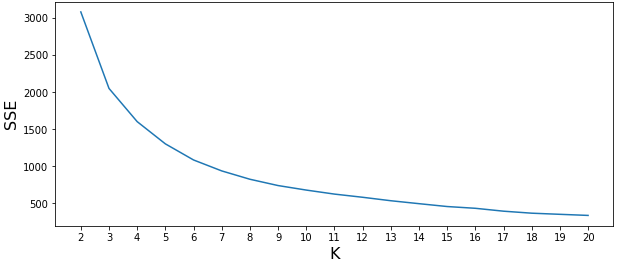
\includegraphics[width=0.45\linewidth]{images/clustering/KMeans/KMeans_K.png}
    \caption{K-Means SSE over K clusters.}
    \label{fig:KMeansK}
\end{figure}
\begin{figure}[H]
    \centering
    \subfloat[K-Means silohuette score]{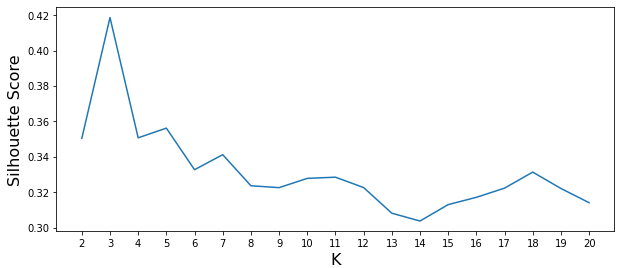
\includegraphics[width=0.45\linewidth]{images/clustering/KMeans/KMeans_Siluette.png}}
    \subfloat[K-Means Davies-Bouldin Score]{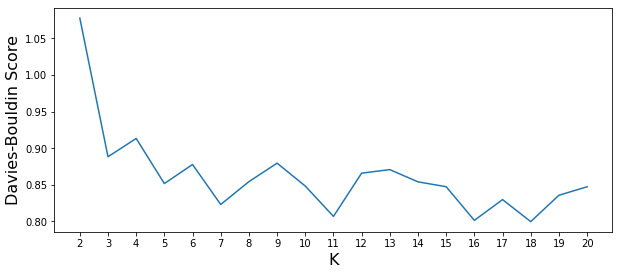
\includegraphics[width=0.45\linewidth]{images/clustering/KMeans/KMeans_Davies.png}}
    \caption{K-Means metrics over k clusters.}
    \label{fig:kmeansMetrics}
\end{figure}

\subsubsection{Cluster analysis}
We applied the PCA on the previously chosen features to analyze the K-means results, then we showed the scatterplot of the first two principal components. As we can see in \autoref{fig:KMeansOut}, the players are divided from left to right by their skills: the weak ones, the average ones and the strong ones. The points on the top right correspond to the top tennis players, such as Djokovic, Nadal and Zverev; we have highlighted Novak Djokovic, the player with rank 1, in the plot to better show the distribution of the players by strength. We have noticed that some players with a high rank are in cluster 0, this is probably due to the fact that they have a high win rate or have won some minor tournaments.

\begin{figure}[H]
    \centering
    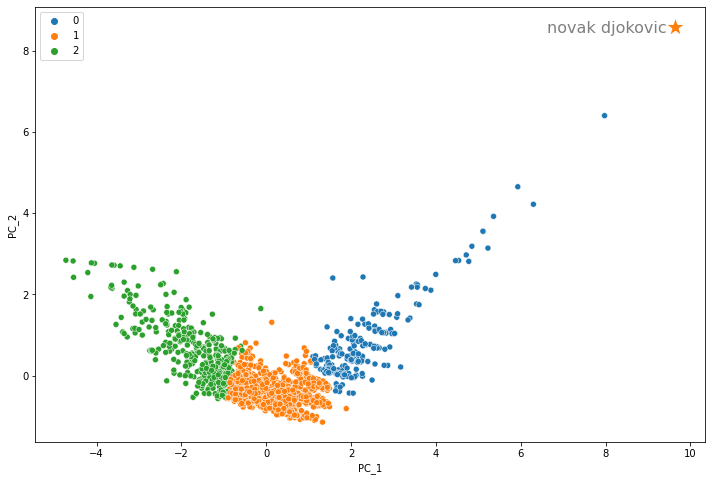
\includegraphics[width=0.5\linewidth]{images/clustering/KMeans/KMeans_out.png}
    \caption{The 3 clusters obtained using K-Means.}
    \label{fig:KMeansOut}
\end{figure}

\begin{figure}[H]
    \centering
    \subfloat{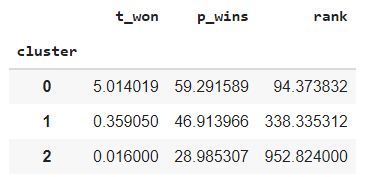
\includegraphics[width=0.30\linewidth]{images/clustering/KMeans/KMeans_stats_avg.png}}
    \subfloat{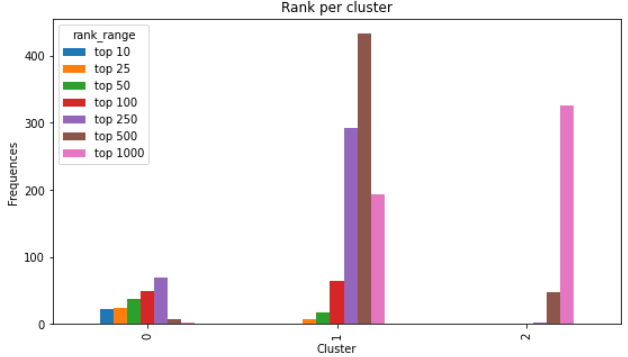
\includegraphics[width=0.3\linewidth]{images/clustering/KMeans/KMeans_stats.png}}
    \caption{Statistics of the feature for each cluster.}
    \label{fig:kmeansAvg}
\end{figure}

\subsection{DBScan}
We decided to work with the dataframe used in the k-means analysis (the one with "t\_won", "p\_wins", "rank"), since we think that it better describes who are the best players and those who aren't.

\subsubsection{Determining eps and min points}
The distance between data points is computed using the Euclidean metric, and for selecting the best eps and min\_samples values we first performed a grid search whose results can be found on the notebook. From the results we choose $min\_samples=8$ and by looking at \autoref{fig:DBScanDist} we choose $eps=0.55$ since it's the value at which the graph's curvature is the highest. The silhouette score is equal to 0.6208

\begin{figure}[H]
    \centering
    \subfloat{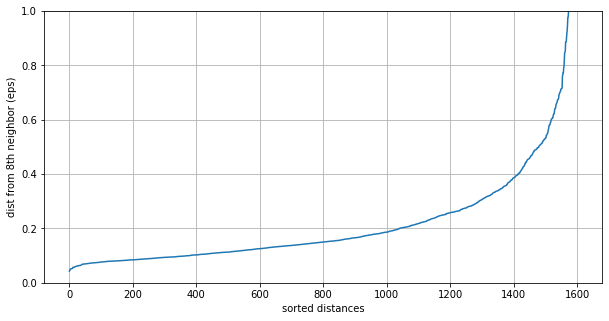
\includegraphics[width=0.45\linewidth]{images/clustering/DBScan/DBScan_dist.png}}
    \subfloat{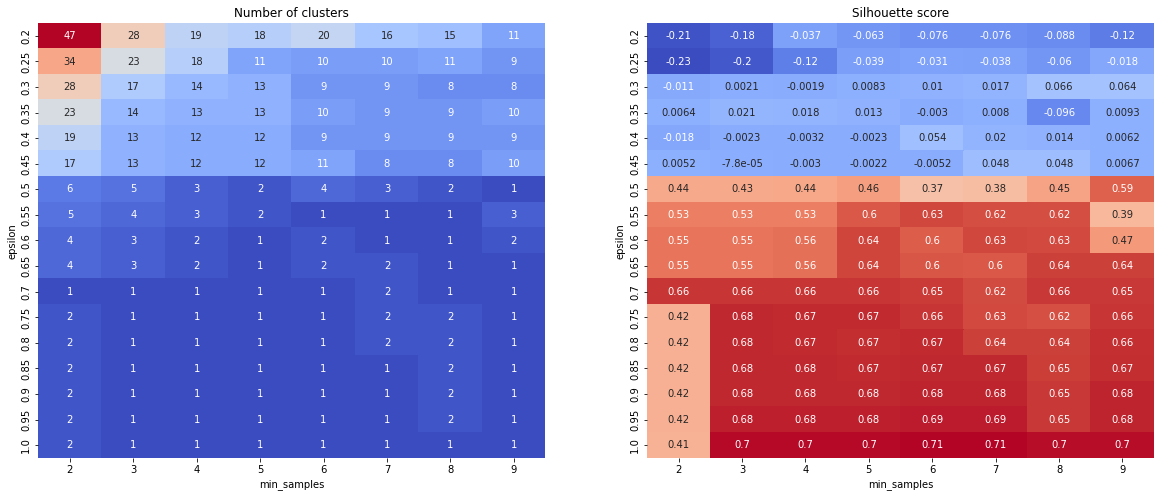
\includegraphics[width=0.55\linewidth]{images/clustering/DBScan/DBScan_grid.png}}
    \caption{DBScan: determining eps and min\_samples}
    \label{fig:DBScanDist}
\end{figure}

\subsubsection{Cluster analysis}
Analyzing the clusters obtained by the DBScan method (\autoref{fig:DBScanOut}), we've seen that there is a single large cluster (the orange one) and the blue points referring to the outliers. In the outliers' cluster there are the players at the extremes: the players who have won very few matches and the strongest players in the world, respectively on the left and right side of the main clsuter. There are also outliers in the center of the plot, representing players who have won some minor tournaments.

\begin{figure}[H]
    \centering
    \subfloat[Clusters generated by applying DBScan, plotted along the 2 P.C.]{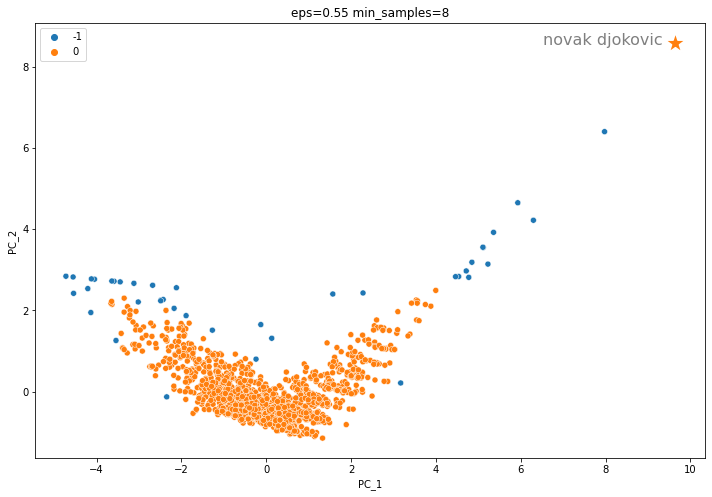
\includegraphics[width=0.52\linewidth]{images/clustering/DBScan/DBScan_out.png}}
    \subfloat[Distribution of players' ranks per cluster]{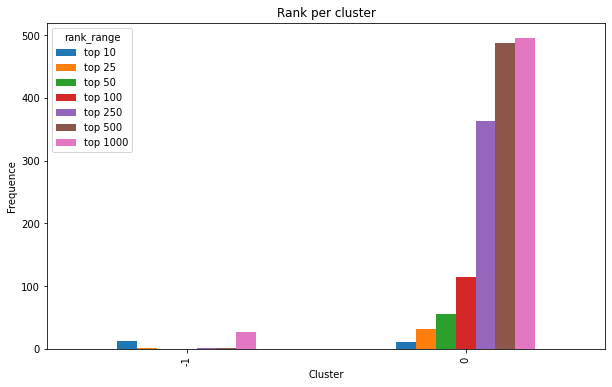
\includegraphics[width=0.48\linewidth]{images/clustering/DBScan/DBScan_rank_clust.png}}
    \caption{DBScan: cluster analysis.}
    \label{fig:DBScanOut}
\end{figure}

\subsection{Hierachical Clustering}
The analysis of the clustering via hierarchical clustering has been conducted using the same set of attributes of the previous algorithms, in order to get results comparable in terms of indicators and properties among the approaches.

\subsubsection{Distance methods}
Like we did with the other clustering algorithms, we used the Euclidean metric to compute the distance between the pairs of points. We have tried several type of agglomerative clustering that differ by the merging criterion of the clusters like min, max, average and ward. In the hierarchical clustering approach, we have not assumed any particular number of clusters: any desired number of clusters can be obtained by ‘cutting’ the dendrogram at the proper level.

\subsubsection{Comparing dendrograms}
\paragraph{Cut threshold} The "best cut" of the dendrograms, is a cut that passes from the longest vertical segment not interrupted by horizontal lines. Anyway we avoided to choose a cut that would have produced too unbalanced clusters.

\begin{table}[H]
\centering
\begin{tabular}{l|l|l}
\textbf{Method}   & \textbf{cluster id : its dimension} & \textbf{Silhouette} \\\hline
Complete & 0: 759, \hspace{2pt} 1: 12, \hspace{2pt} 2: 827, \hspace{2pt} 3: 2 & 0.3082\\
Single   & 0: 1598, 1: 1, \hspace{2pt} \hspace{2pt} 2: 1 & 0.8013 \\
Average  & 0: 1580, 1: 2, \hspace{2pt} \hspace{2pt} 2: 18 & 0.6485 \\
Ward     & 0: 330, \hspace{2pt} 1: 296, 2: 974 & 0.3756 \\\hline  
\end{tabular}
\end{table}
Even if the silhouette is pretty good using the single and average methods, we can not say the same thing looking at the dendrograms, since the clusters are unbalanced, and as a consequence, most of the points falls in one big cluster. The only exceptions in this behaviour is produced by applying Ward method, that produced an almost balanced clusters closer to the K-Means ones, as shown in \autoref{fig:hier_clusters}.

\begin{figure}[H]
    \centering
    \subfloat[Complete]{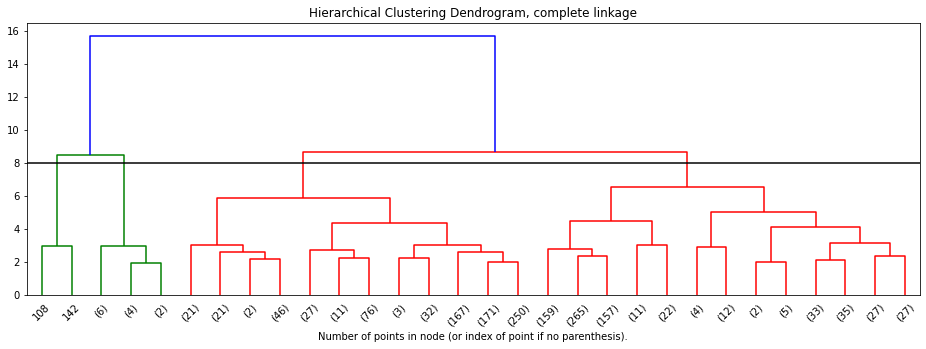
\includegraphics[width=0.5\linewidth]{images/clustering/Hierarchical/Hierac_complete.png}}
    \subfloat[Single]{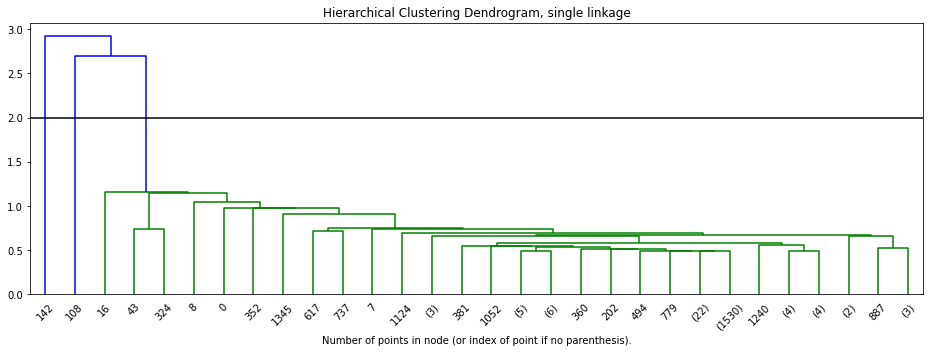
\includegraphics[width=0.5\linewidth]{images/clustering/Hierarchical/Hierac_single.png}}\\
    \subfloat[Average]{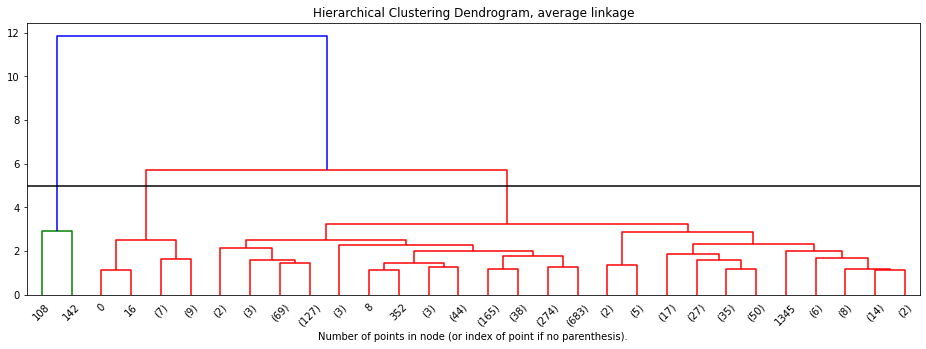
\includegraphics[width=0.5\linewidth]{images/clustering/Hierarchical/Hierac_avg.png}}
    \subfloat[Ward]{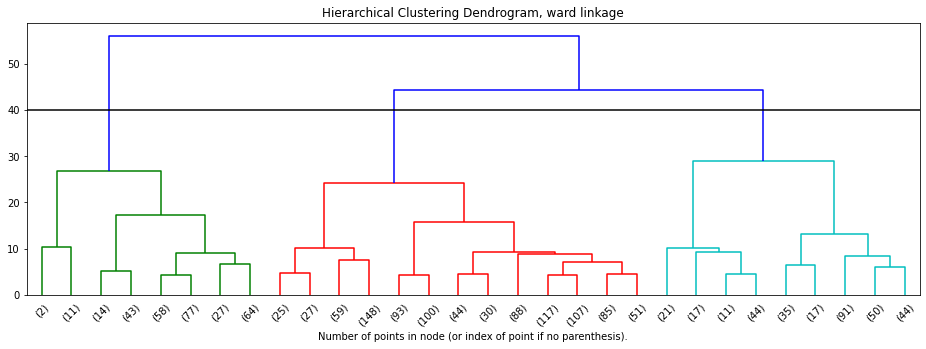
\includegraphics[width=0.5\linewidth]{images/clustering/Hierarchical/Hierac_ward.png}}
    \caption{Hierarchical clustering methods comparison: dendrograms.}
    \label{fig:hier_dendograms}
\end{figure}

\subsubsection{Comparing clusters}
By looking at the pcas plot from \autoref{fig:hier_clusters}, we can define the hierarchical clusterings with complete and ward linkage as the best ones among the four methods. The single linkage was the worst one since it created two cluster with one player each (Djokivic and Nadal which are the best overall player), meanwhile the average one separated the extremely strong players (again Djokivic and Nadal) from the strong ones (green cluster) and the average or weak ones (blue cluster). The only approach that didn't have such drastic separation were the complete and ward linkages, which is why we considered them as the best among foru approaches.
\begin{figure}[H]
    \centering
    \subfloat[Complete]{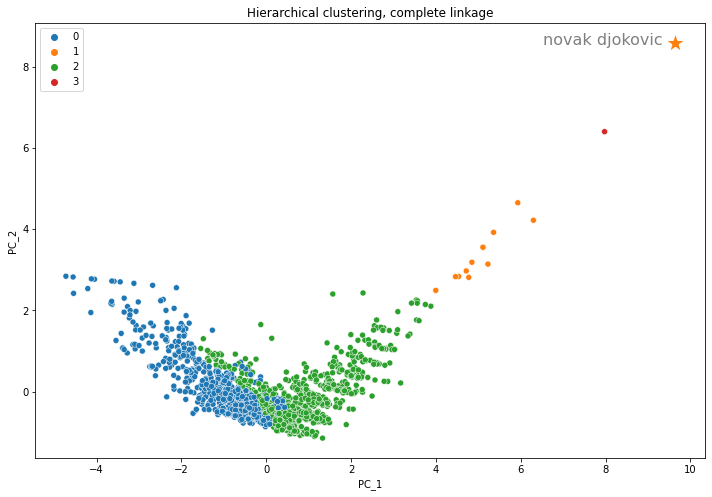
\includegraphics[width=0.4\linewidth]{images/clustering/Hierarchical/Hierac_complete_cluster.png}}
    \subfloat[Single]{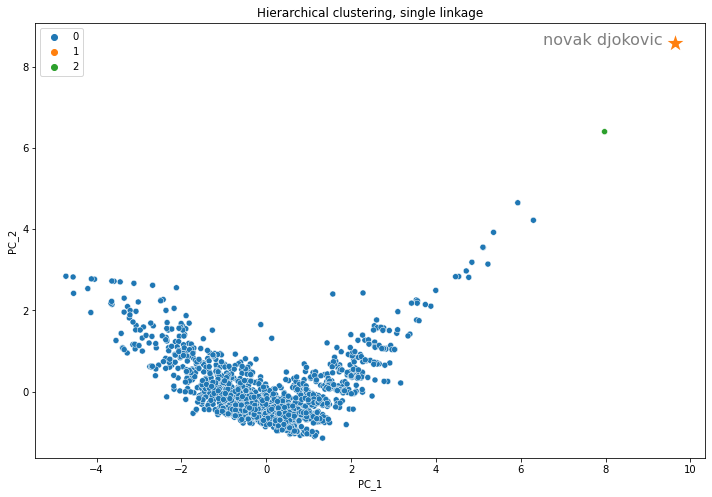
\includegraphics[width=0.4\linewidth]{images/clustering/Hierarchical/Hierac_single_cluster.png}}\\
    \subfloat[Average]{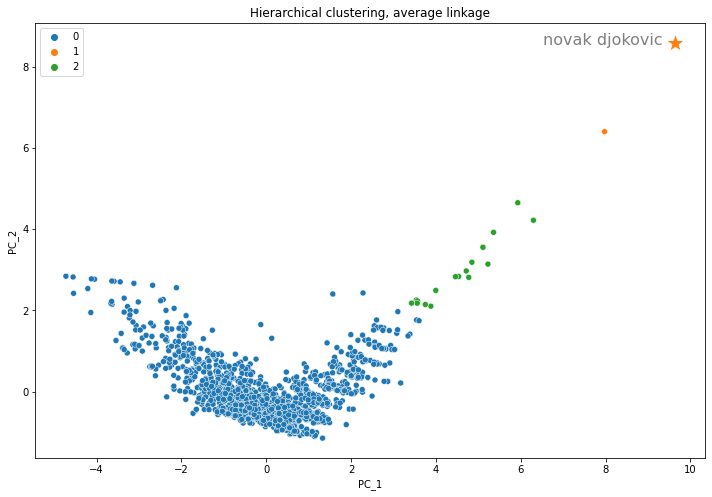
\includegraphics[width=0.4\linewidth]{images/clustering/Hierarchical/Hierac_avg_cluster.png}}
    \subfloat[Ward]{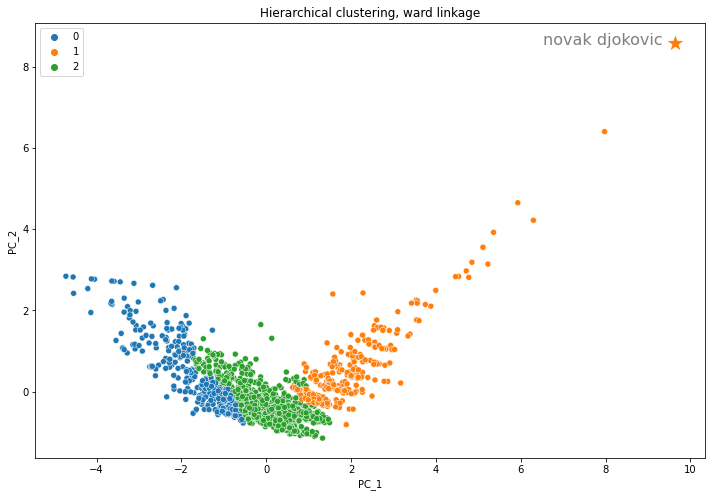
\includegraphics[width=0.4\linewidth]{images/clustering/Hierarchical/Hierac_ward_cluster.png}}
    \caption{Hierarchical clustering: plotting along the PCAs.}
    \label{fig:hier_clusters}
\end{figure}

\subsection{Validation by external measures}
We computed the \textit{similarity matrix} $S$ given a particular clustering. To obtain this matrix, the indices are sorted according to the labels of the clusters and the component $S(i,j)$ is equal to $e^{-d(i,j)}$, where $d(i,j)$ is the euclidean distance between the points $i$ and $j$. If we have well-separated clusters, then the similarity matrix should be roughly block-diagonal. We also computed the entropy of each feature per cluster: a low entropy score of each attribute indicates a more predictable and less uncertain trend within the clusters. 

\begin{figure}[H]
    \centering
    \subfloat[Similarity Kmeans]{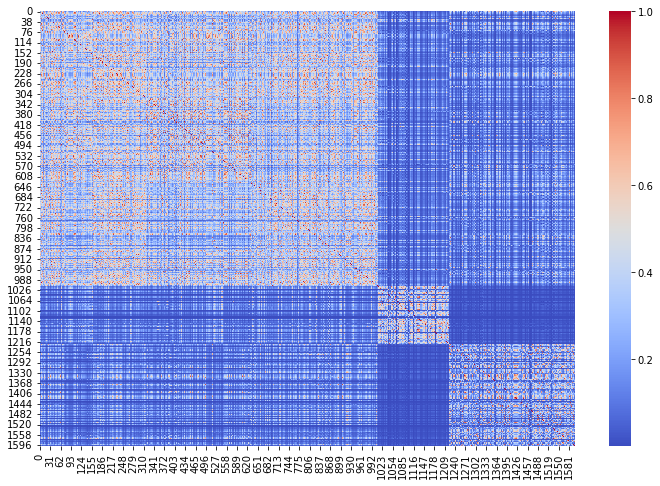
\includegraphics[width=0.3\linewidth]{images/clustering/Validation/KmeansSimMatrix.png}}
    \subfloat[Entropy Kmeans]{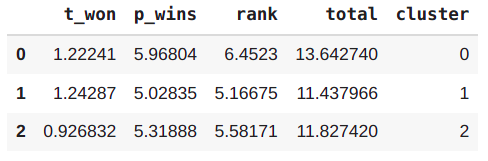
\includegraphics[width=0.3\linewidth]{images/clustering/Validation/kmeansEntropy.png}}\\
    \subfloat[Similarity\\Complete]{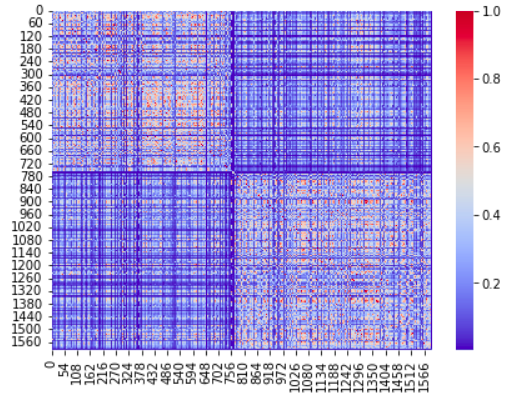
\includegraphics[width=0.3\linewidth]{images/clustering/Validation/completeSimMatrix.png}}   
    \subfloat[Entropy Complete]{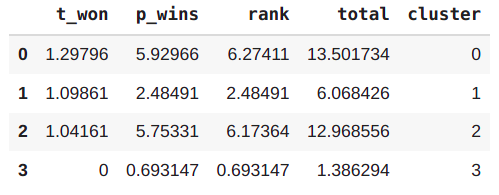
\includegraphics[width=0.3\linewidth]{images/clustering/Validation/completeEntropy.png}}\\
    \subfloat[Similarity\\Ward]{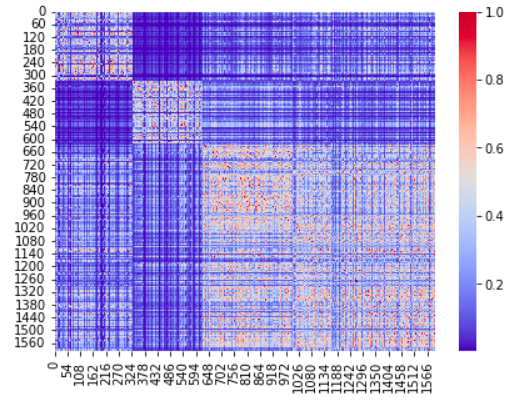
\includegraphics[width=0.3\linewidth]{images/clustering/Validation/SimWard.png}}   
    \subfloat[Entropy Ward]{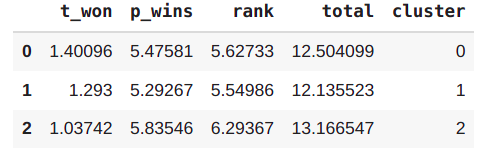
\includegraphics[width=0.3\linewidth]{images/clustering/Validation/EntropyWard.png}}\\
    \subfloat[Entropy Single]{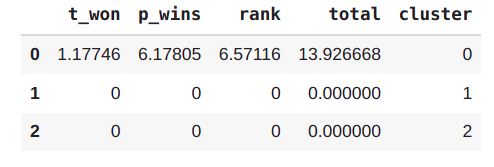
\includegraphics[width=0.3\linewidth]{images/clustering/Validation/EntropySingle.png}}
    \subfloat[Entropy Average]{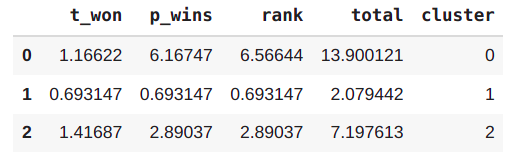
\includegraphics[width=0.3\linewidth]{images/clustering/Validation/EntropyAv.png}}
    \caption{Similarity matrices and Entropy of attributes per cluster for each method}
    \label{fig:val_clusters}
\end{figure}

\iffalse
We compute the \textit{cross-correlation} between the \textit{similarity matrix} of the clustering and the \textit{incidence matrix} (where the component $(i, j)$ is equal to $1$ if $i$ and $j$ are in the same cluster, $0$ otherwise). The \textit{incidence matrix} represents the similarity matrix of a perfect clustering, so high-values component of the cross-correlation matrix represents an high correlation of the two matrix in that offset.
\fi

\subsection{Other Clustering approaches explored}
For the final work on clustering we went to explore two more approaches from the pyclustering package as suggested by the professor, our choice fell on X-Means and SOM soft-clustering.
\subsubsection{X-Means}
From the pyclustering package documentation: X-means clustering method starts with the assumption of having a minimum number of clusters, and then dynamically increases them. X-means uses specified splitting criterion to control the process of splitting clusters.
\vspace{3mm}

This approach is different from the previous ones we tried, since it doesn't need to know beforehand the number of clusters, but it starts with a pre-determined amount and then splits them into smaller ones. The results change from one try to another, but we've seen that this approach usually worked better for our dataframe.
\begin{figure}[H]
    \centering
    \subfloat[Clusters generated by X-Means]{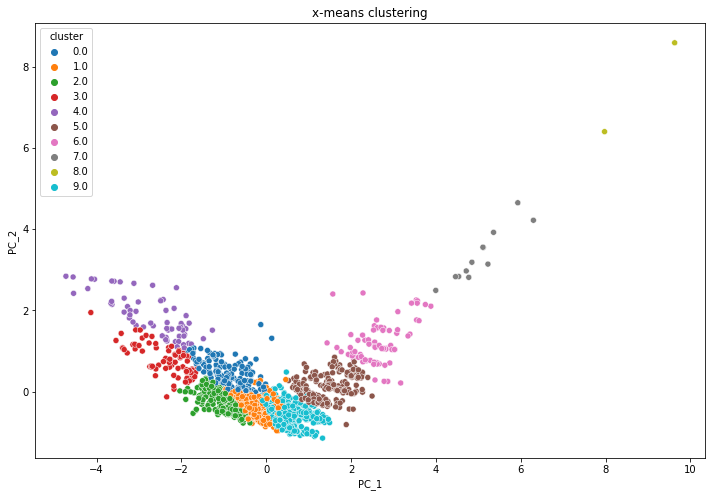
\includegraphics[width=0.38\linewidth]{images/clustering/OtherClusterings/x_means_pca.png}}
    \subfloat[Distribution of players' ranks per cluster]{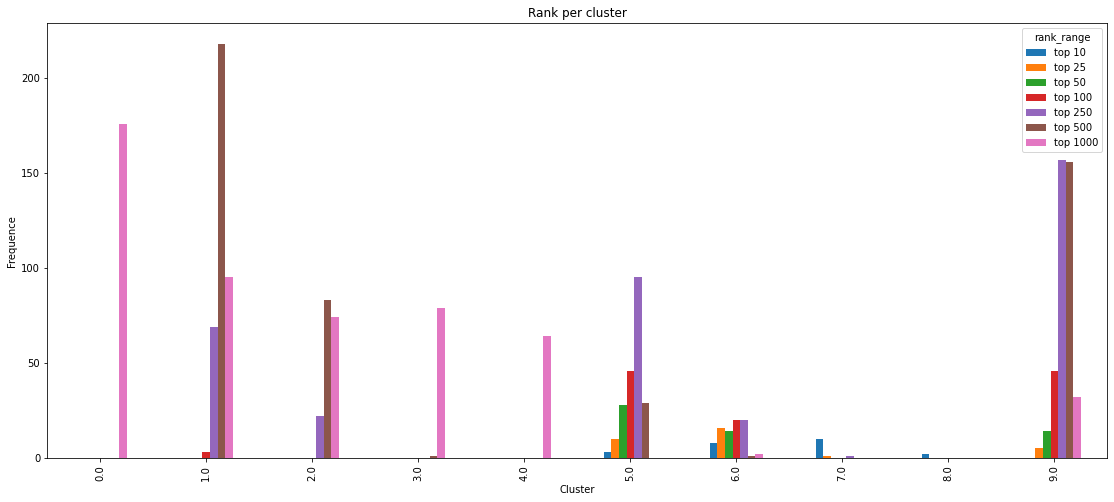
\includegraphics[width=0.62\linewidth]{images/clustering/OtherClusterings/x_means_ranks.png}}
    \caption{X-Means: pca and analysis.}
    \label{fig:x_means}
\end{figure}

By looking at \autoref{fig:x_means} we can see that X-Means separated better the players by their skills than our previous attempts, so we think that it did the best job among everything we tried.

\subsubsection{SOM Soft-Clustering}
From the pyclustering package documentation: this algorithm uses an amount of clusters that should be allocated as the size of a SOM map. The captured objects by the neurons are clusters. We expected the pyclustering library to provide us a way to plot the SOM lattice but this wasn't the case, so we went, as always, with the pca just like the other approaches. For the choice of k we did the same work as K-Means and we found that the best choice was for $k=3$ but we couldn't calculate in any way the SSE since the implementation by the library doesn't come with a way to obtain the cluster centroids, so we only considered the Silhoutte and Davies-Bouldin scores.

\begin{figure}[H]
    \centering
    \subfloat[Clusters generated by SOMsc]{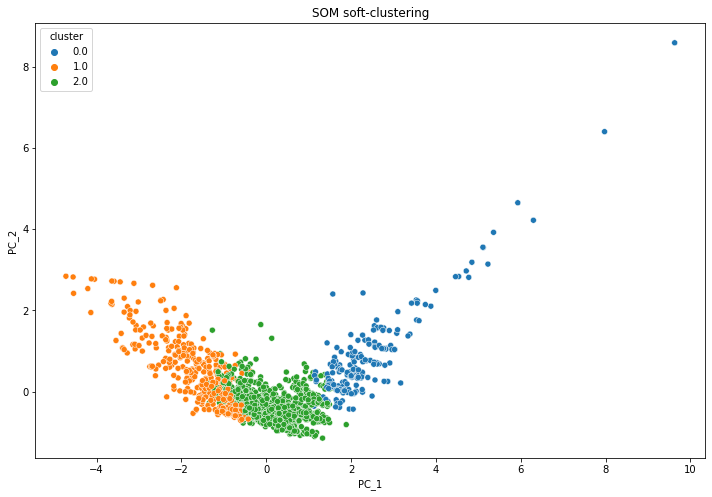
\includegraphics[width=0.48\linewidth]{images/clustering/OtherClusterings/somsc_pca.png}}
    \subfloat[Distribution of players' ranks per cluster]{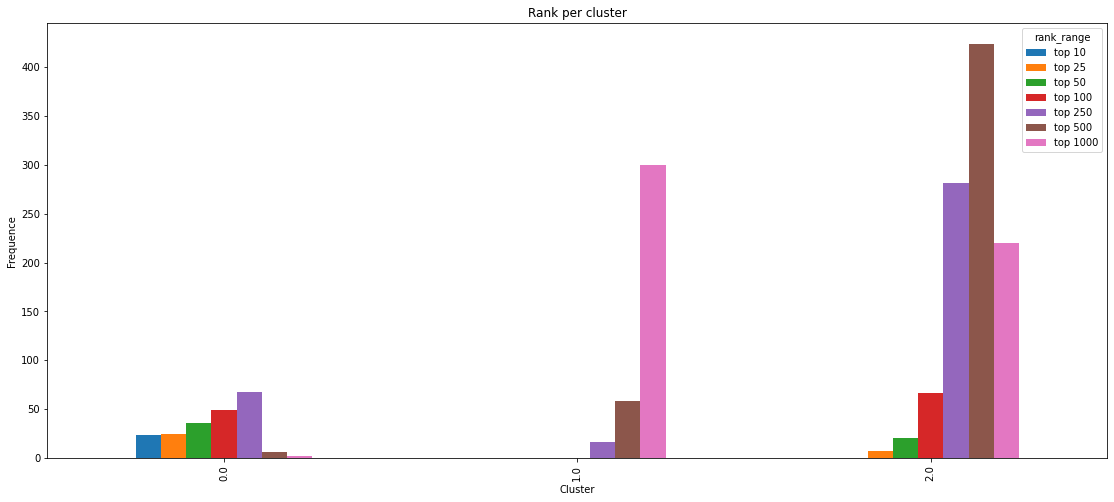
\includegraphics[width=0.52\linewidth]{images/clustering/OtherClusterings/somsc_ranks.png}}
    \caption{SOM soft-clusering: plot along PCAs and analysis.}
    \label{fig:somsc}
\end{figure}

The results obtained, which can be seen on \autoref{fig:somsc}, are similar to the ones obtained by k-means, so we think we don't need to explain anything more about this approach.
\end{document}
